\chapter{Methodology}

\section{Overview: the pipeline in eight steps}

This chapter follows the running example, one chest CT and its caption, through the model in the order the data flows (Figure 3.1).

\textbf{Encoder (Steps 1--5):} turns the image into 49 summary vectors.

\begin{enumerate}
\def\labelenumi{\arabic{enumi}.}
\tightlist
\item
  \textbf{Image → patch tokens:} the scan is cut into small patches, and each patch becomes a vector (3.3).
\item
  \textbf{Swin block:} LayerNorm, attention and an MLP update the tokens (3.4).
\item
  \textbf{Window attention:} tokens exchange information inside \(7 \times 7\) windows (3.5).
\item
  \textbf{Shifted windows:} every second block shifts the windows so neighbouring windows connect (3.6).
\item
  \textbf{Patch merging and four stages:} the grid of tokens shrinks from \(56 \times 56\) to \(7 \times 7\), giving the \textbf{image memory} \(Z\) (3.7).
\end{enumerate}

\textbf{Decoder (Steps 6--8):} turns \(Z\) into a caption.

\begin{enumerate}
\def\labelenumi{\arabic{enumi}.}
\setcounter{enumi}{5}
\tightlist
\item
  \textbf{Caption → decoder input:} word embedding, positional encoding and teacher forcing (3.8).
\item
  \textbf{Decoder layers:} masked self-attention reads the earlier words; cross-attention reads the image (3.9).
\item
  \textbf{Output and generation:} softmax gives next-word probabilities; beam search chooses the caption (3.10).
\end{enumerate}

\textbf{Training} follows in Section 3.11. Attention is used in Steps 3, 4 and 7, so Section 3.2 explains it first.

\begin{figure}
\centering
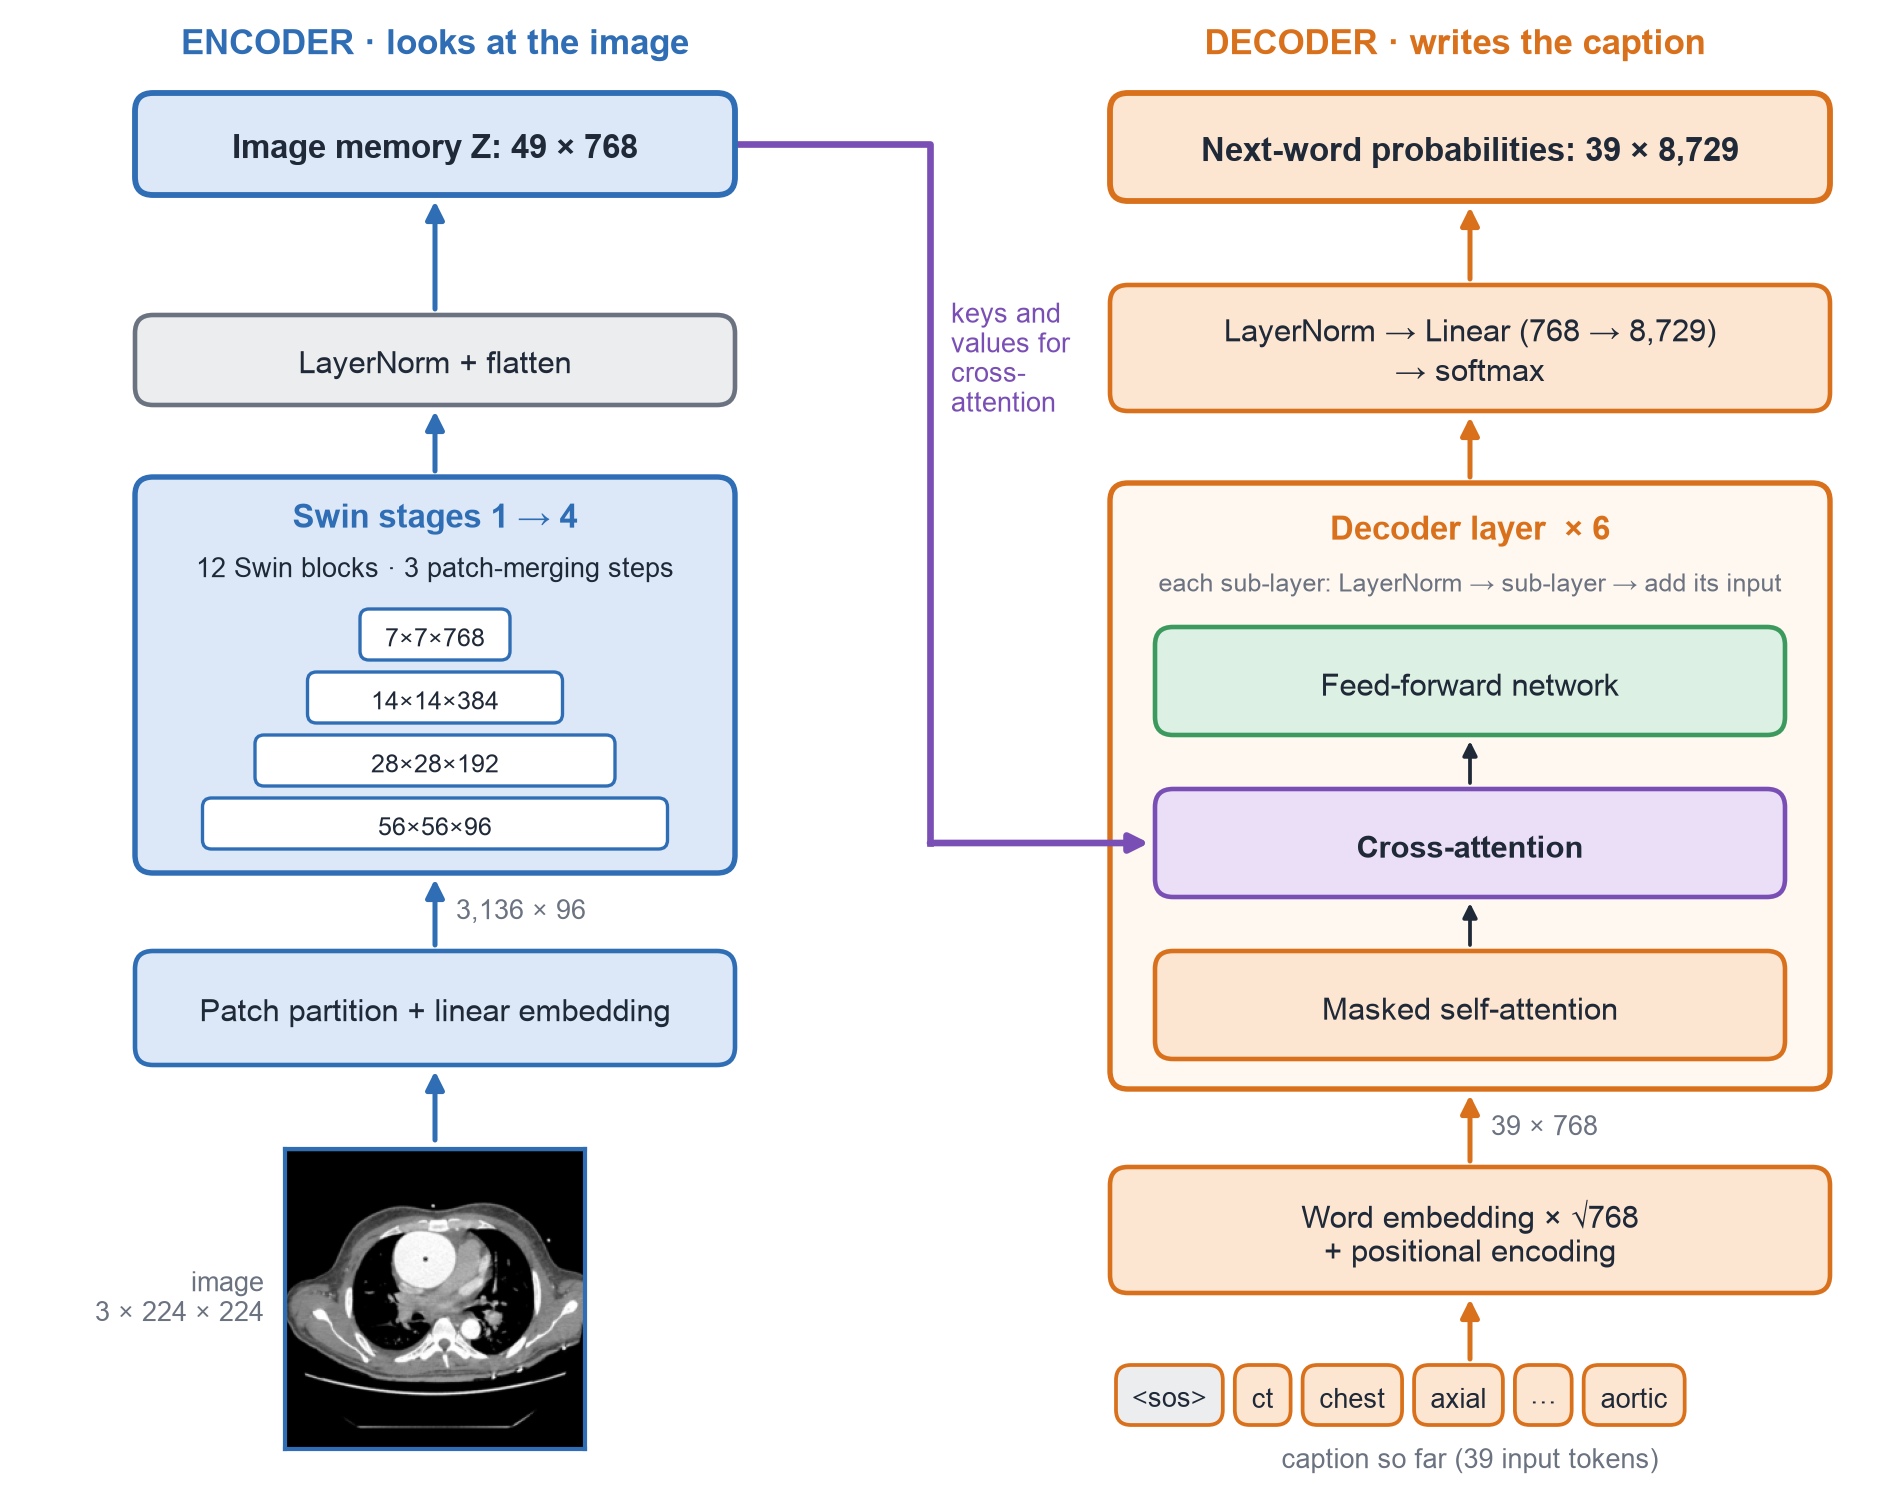
\includegraphics[width=0.7\linewidth,height=\textheight,keepaspectratio]{figures/fig3_1_overall.png}
\caption{The full model. Left: the Swin-T encoder turns the image into the image memory Z. Right: the Transformer decoder turns the caption written so far into next-word probabilities, reading Z through cross-attention in each of its six layers.}
\end{figure}

\needspace{20\baselineskip}

\begin{longtable}[]{@{}
  >{\raggedright\arraybackslash}p{(\linewidth - 4\tabcolsep) * \real{0.3333}}
  >{\raggedright\arraybackslash}p{(\linewidth - 4\tabcolsep) * \real{0.3333}}
  >{\raggedright\arraybackslash}p{(\linewidth - 4\tabcolsep) * \real{0.3333}}@{}}
\caption{Notation and sizes used in this chapter.}\tabularnewline
\toprule\noalign{}
\begin{minipage}[b]{\linewidth}\raggedright
Symbol
\end{minipage} & \begin{minipage}[b]{\linewidth}\raggedright
Meaning
\end{minipage} & \begin{minipage}[b]{\linewidth}\raggedright
Value in our model
\end{minipage} \\
\midrule\noalign{}
\endfirsthead
\toprule\noalign{}
\begin{minipage}[b]{\linewidth}\raggedright
Symbol
\end{minipage} & \begin{minipage}[b]{\linewidth}\raggedright
Meaning
\end{minipage} & \begin{minipage}[b]{\linewidth}\raggedright
Value in our model
\end{minipage} \\
\midrule\noalign{}
\endhead
\bottomrule\noalign{}
\endlastfoot
\(B\) & Batch size & 32 \\
\(H_s \times H_s\) & Token grid at encoder stage \(s\) & \(56^2,\allowbreak\ 28^2,\allowbreak\ 14^2,\allowbreak\ 7^2\) \\
\(C_s\) & Numbers per token at stage \(s\) & 96, 192, 384, 768 \\
\(M\) & Window size (tokens per side) & 7 \\
\(h\), \(d\) & Attention heads, numbers per head & encoder: 3--24 heads × 32; decoder: 8 heads × 96 \\
\(Z\) & Image memory (encoder output) & \(49 \times 768\) \\
\(T\) & Caption length in tokens & 40 (39 decoder positions) \\
\(\lvert V \rvert\), \(E\) & Vocabulary size, embedding table & 8,729; \(8{,}729 \times 768\) \\
\end{longtable}

\section{Attention: the core operation}

\textbf{What it does.} Attention lets each token update itself using information from other tokens. Every token produces three vectors:

\begin{itemize}
\tightlist
\item
  a \textbf{query} (\(q\)): ``what am I looking for?'';
\item
  a \textbf{key} (\(k\)): ``what do I contain?'';
\item
  a \textbf{value} (\(v\)): ``what do I pass on?''.
\end{itemize}

A token compares its query with every key. The better the match, the more of that token's value it takes, so the result is a weighted average of the values.

\begin{intuitionbox}

\textbf{Everyday comparison: a library search.} Your question is the query, the titles on the book spines are the keys, and the contents of the books are the values. You read mostly the books whose titles match your question best.

\end{intuitionbox}

\textbf{The math.} For input tokens \(X\) (and, in cross-attention, a second set of tokens \(X'\) that supplies the keys and values):

\[Q = X W_Q, \qquad K = X' W_K, \qquad V = X' W_V \tag{3.1}\]

\[\text{Attention}(Q, K, V) = \text{softmax}\left(\frac{Q K^\top}{\sqrt{d}} + B\right) V \tag{3.2}\]

where:

\begin{itemize}
\tightlist
\item
  \(W_Q\), \(W_K\) and \(W_V\) are learned matrices;
\item
  \(d\) is the number of numbers per head;
\item
  \(B\) is an optional term: a position bias, or a mask that blocks some pairs;
\item
  softmax turns each row of scores into positive weights that sum to 1.
\end{itemize}

\begin{figure}
\centering
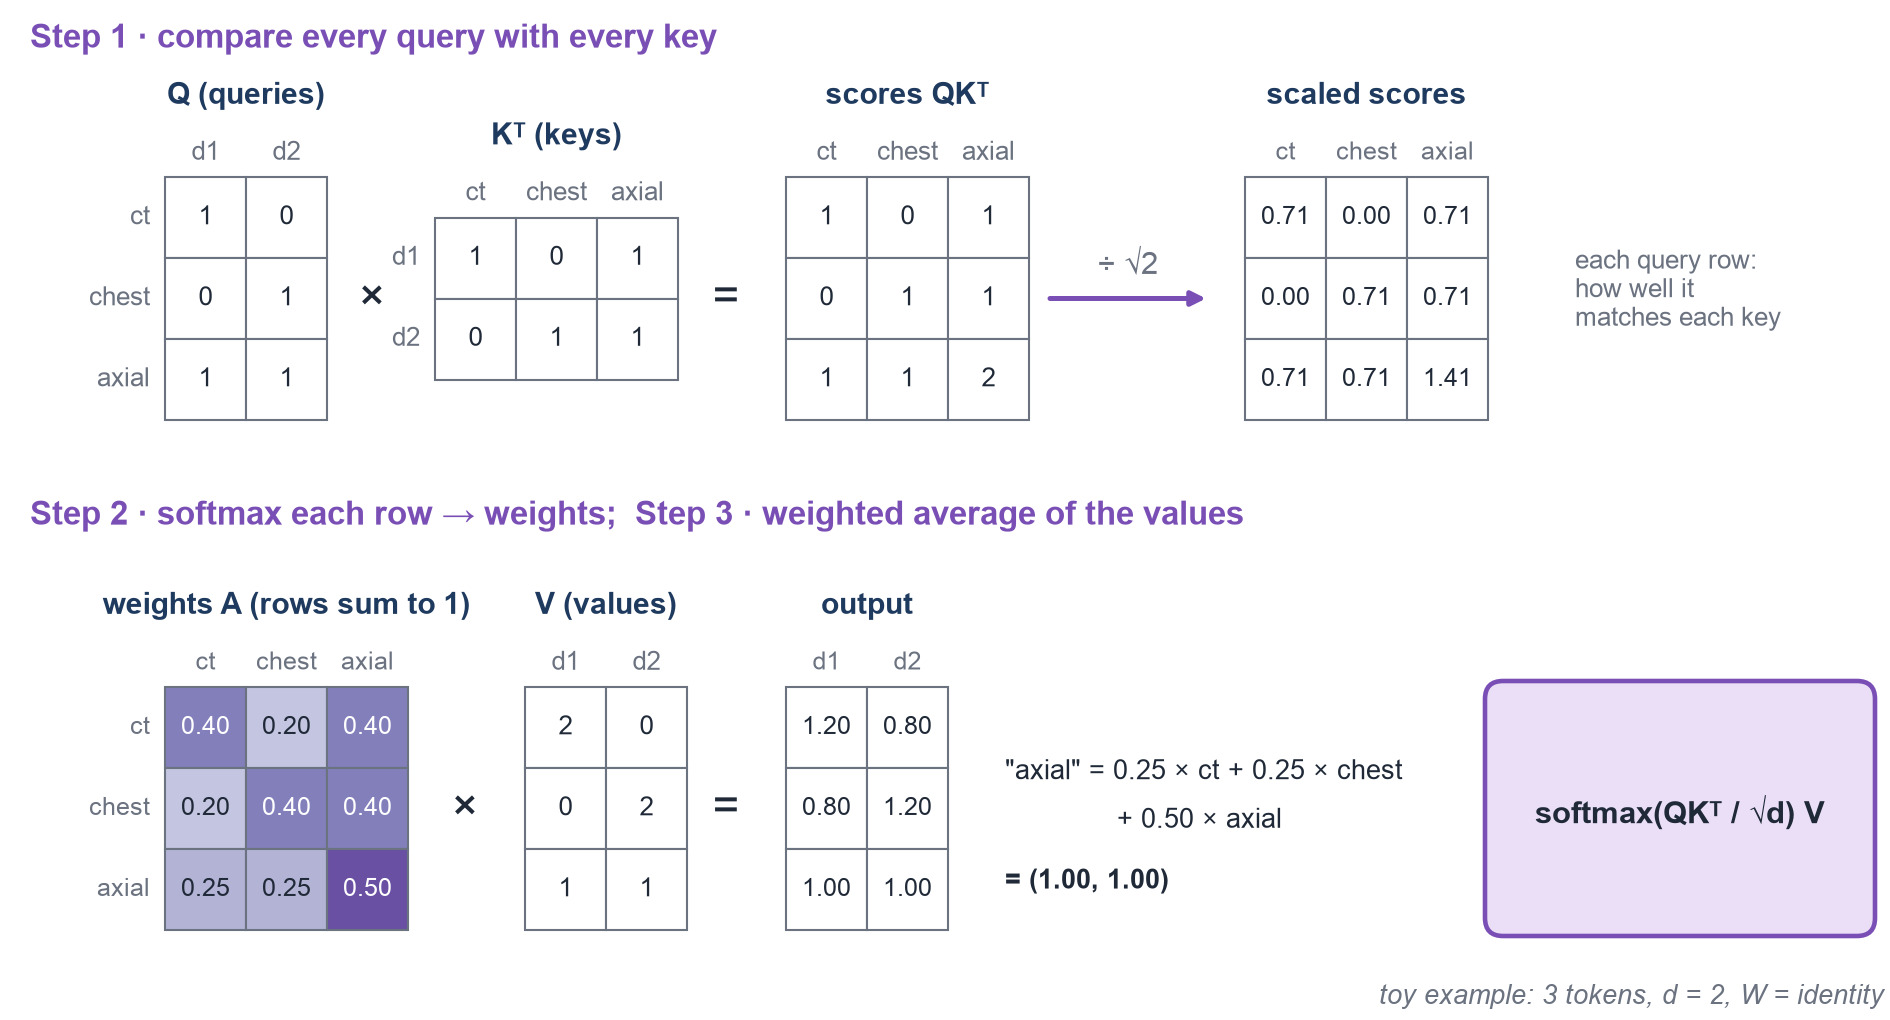
\includegraphics[width=1\linewidth,height=\textheight,keepaspectratio]{figures/fig3_25_attention_steps.png}
\caption{Attention computed step by step for three tokens with d = 2. Step 1 compares queries with keys; step 2 turns each row into weights with softmax; step 3 averages the values with those weights.}
\end{figure}

\begin{examplebox}

\textbf{Worked example (Figure 3.2).} The query of ``axial'' is \((1,\allowbreak 1)\).

\textbf{Scores.} Compared with the keys of (ct, chest, axial), it scores \((1,\allowbreak 1,\allowbreak 2)\), or \((0.71,\allowbreak 0.71,\allowbreak 1.41)\) after dividing by \(\sqrt{2}\).

\textbf{Weights.} Softmax gives \((0.25,\allowbreak 0.25,\allowbreak 0.50)\).

\textbf{Output.} \(0.25 \times (2,\allowbreak 0) + 0.25 \times (0,\allowbreak 2) + 0.50 \times (1,\allowbreak 1) = (1.00,\allowbreak\ 1.00)\): a blend of all three values that leans towards ``axial'' itself.

\end{examplebox}

\textbf{Why divide by \(\sqrt{d}\)?} A dot product of two random \(d\)-number vectors grows roughly like \(\sqrt{d}\): about 1.4 for \(d = 2\) but 9.8 for \(d = 96\). Without scaling, softmax would give almost all the weight to one key. For example, the scores \((1.0,\allowbreak 0.5,\allowbreak 0.2,\allowbreak -0.3)\) multiplied by 9.8 give weights \((0.99,\allowbreak 0.01,\allowbreak 0.00,\allowbreak 0.00)\), while the scaled scores give \((0.43,\allowbreak 0.26,\allowbreak 0.19,\allowbreak 0.12)\).

\textbf{Multi-head attention.} The \(C\) numbers of each token are split into \(h\) \textbf{heads} of \(d = C/h\) numbers. Each head computes its own attention, so it can look for a different kind of relationship. The heads' results are joined and mixed by a final linear layer:

\[\text{MHA}(X) = \left[\text{head}_1 ;\ \ldots ;\ \text{head}_h\right] W_O \tag{3.3}\]

Attention is used in four ways in this model (Figure 3.3). Each is worked through with numbers where it first appears:

\begin{itemize}
\tightlist
\item
  \textbf{Window self-attention:} Section 3.5.
\item
  \textbf{Shifted-window attention:} Section 3.6.
\item
  \textbf{Masked self-attention and cross-attention:} Section 3.9.
\end{itemize}

\begin{figure}
\centering
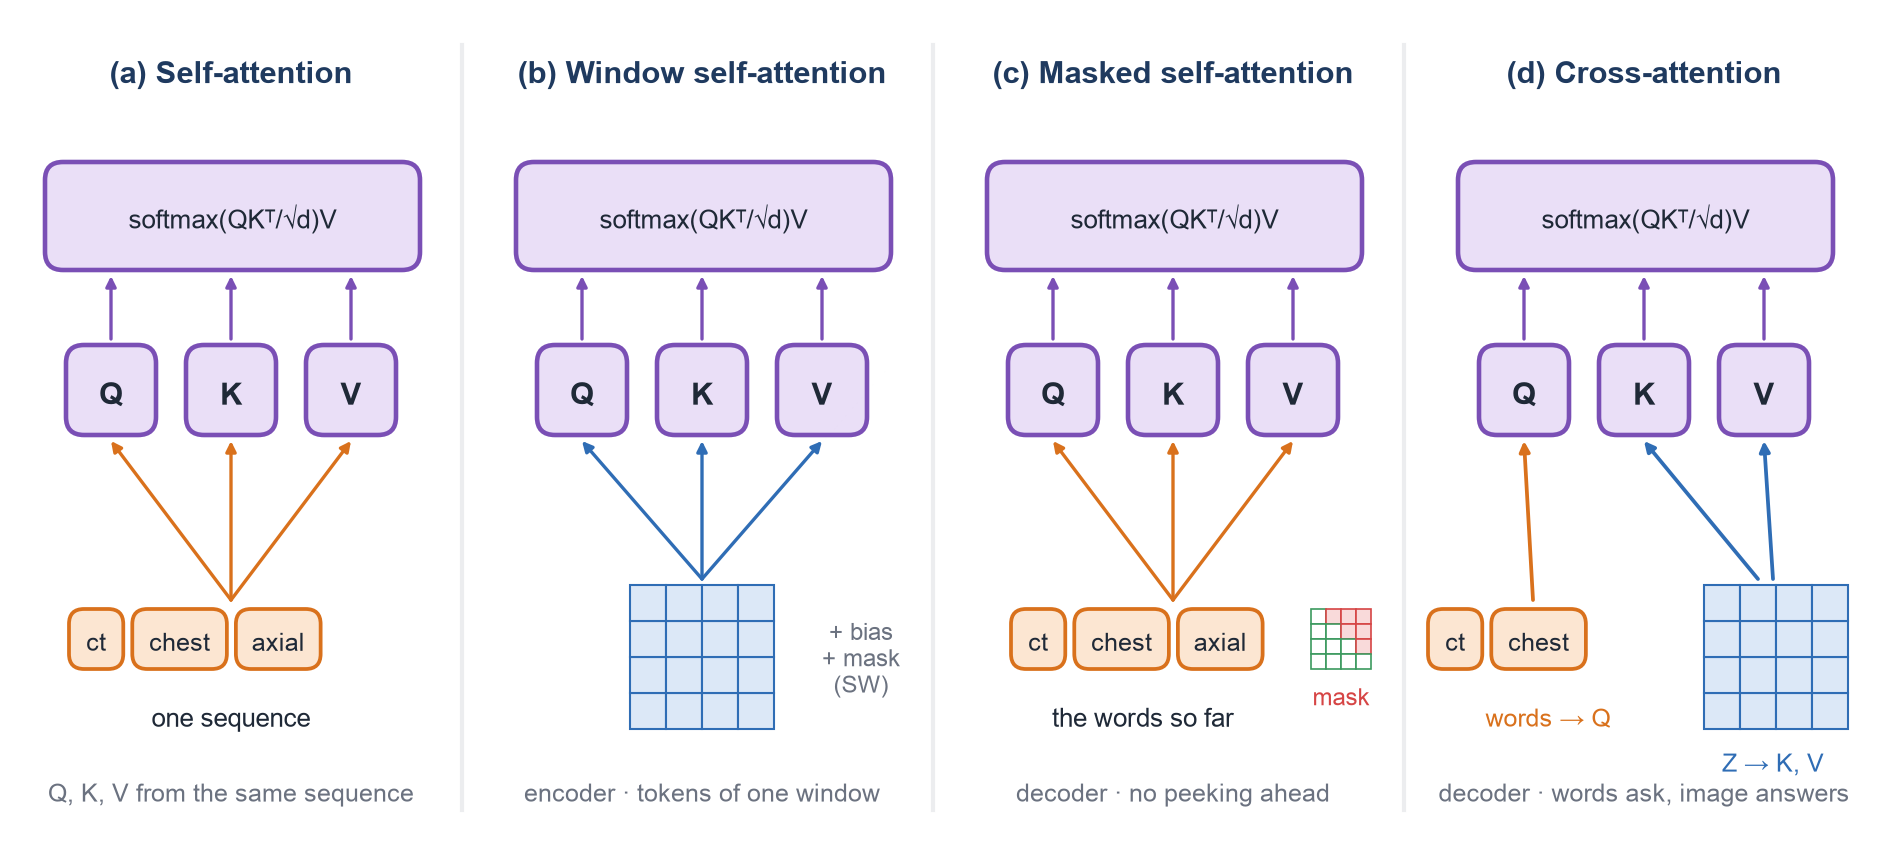
\includegraphics[width=1\linewidth,height=\textheight,keepaspectratio]{figures/fig3_27_qkv_sources.png}
\caption{The four types of attention in the model, and where their queries, keys and values come from.}
\end{figure}
